Programmet MatLabb har i stort tre delsystem:

\begin{enumerate}
\item \verb+GUI+, Det grafiska användargränssnittet
\item \verb+Shell+, eller, det inre skalet som håller centrala objekt och variabler, t.ex. aktivt recept och portionskalning.
\item \verb+Lookup+, som tillhandahåller relevanta verktyg för kommunikation med databasen.
\end{enumerate}
\verb+GUI+ ansvarar för att skriva ut data från det inre systemet på skärmen i grafisk tappning. Användaren styr även systemet genom att interagera med menyer, knappar och strängfält snarare än att ge skriftliga hänvisningar till kommandoprompten. Information presenteras enligt konceptbilderna i (figur \ref{fig:vy1} - \ref{fig:vy4}). Det grafiska gränssnittet implementeras med hjälp av biblioteket Qt och kommer delvis designas i klienten Qt Creator.

\section{Shell}
\verb+Shell+ innehåller objekt av klasserna \verb+Recipe+, \verb+InfoIngredient+ och \verb+Lookup+ som datamedlemmar, där de två förstnämnda reflekterar det aktuella receptet och ingrediensen som vårt program interagerar med. Utåt tillhandahåller \verb+Shell+ publikt endast funktioner som kan tänkas motsvara alla möjliga handlingar från användaren. Denna grupp av funktioner inkluderar, men är ej begränsade till, funktionerna listade i figur \ref{fig:tekfunklist} (s. \pageref{fig:tekfunklist}).

\begin{figure}[h]
\caption{Funktioner för användarinputs}
\begin{tabular}{p{5.5cm}|p{8cm}}
\verb+addRecipe(string+) & Konstruerar ett nytt tomt \verb+Recipe+-objekt för datamedlemmen \verb+currentRecipe_+. Ett defaultargument av datatypen string existerar för att potentiellt tilldela ett namn. \\[1.2mm]
\verb+editRecipe()+ & Kallar på \verb+currentRecipe_.editRecipe()+ för att kunna ändra på dess datamedlemmar.\\[1.2mm]
\verb+importTxt(string)+ & Importering från textfil. Konstruerar ett nytt \verb+Recipe+-objekt och försöker fylla i dess datamedlemmar enligt en standardmodell.\\[1.2mm]
\verb+exportTxt()+ & Kallar på \verb+currentRecipe_.exportTxt(string)+ för att exportera till .txt. Kan modifieras för att först hämta ett annat recept från databasen för exportering.\\[1.2mm]
\verb+addIngredient(string)+ & Motsvarande \verb+addRecipe+. \\[1.2mm]
\verb+editIngredient(string)+ &  Motsvarande \verb+addIngredient+. \\[1.2mm]
\verb++&\\[1.2mm]
\verb+matchRecipe(string)+ & Levererar en sträng till \verb+Lookup+-objektet för att slå i databasen för exakt matchning. \\[1.2mm]
\verb+matchIngredient(string)+ &  Motsvarande \verb+matchRecipe+. \\[1.2mm]
\verb+searchRecipe(cont<SearchTerm*>)+ & Levererar söktermer i en godtycklig container till \verb+Lookup+. \verb+recipeSearchResults_+ tilldelas det resultat som \verb+Lookup+ ger.  \\[1.2mm]
\verb++&\\[1.2mm]
\verb++& get-funktioner som används av GUI:t och returnerar relevant data. 
\end{tabular}
\label{fig:tekfunklist}
\end{figure}

\subsection{Recipe \& InfoIngredient}
Objekt av klasserna \verb+Recipe+ och \verb+InfoIngredient+ kommer endast att existera i stabilt tillstånd som datamedlemmar i klassen \verb+Shell+. Nya objekt skapas antingen i samband med t.ex. funktionen \verb+addRecipe(string)+ eller byggs upp och returneras av \verb+Lookup+ som resultat av en matchning i databasen. Klasserna \verb+Recept+ och \verb+InfoIngredient+ innehåller främst fullständig data om ett specifikt recept/ingrediens, men även funktioner för implementeringen av \verb+Shell+s ``användarfunktioner'', t.ex. åtkomst och redigering. Lista över datamedlemmar i klassen \verb+Recipe+:
 
%Figure: tabular
\begin{itemize}
\item \verb+string name_+ - \emph{Namn på receptet}
\item \verb+string description_+ - \emph{Beskrivning/utförande}
\item \verb+int minutesTime_+ - \emph{Tidsåtgång i minuter}
\item \verb+cont<string> comments_+ - \emph{Kommentarer i godtycklig container}
\item \verb+"referens" image_+ - \emph{Någon typ av referens för implentering av tillhörande bilder}
\item \verb+double grade_+ - \emph{Betyg}
\end{itemize}

\begin{itemize}
\item \verb+cont<RecipeIngredient> ingredients_+ - \emph{Ingredienser som ingår}
\item \verb+cont<RelatedRecipe> relatedRecipes_+ - \emph{Besläktade recept}
\end{itemize}
%end
%
\verb+InfoIngredient+ och \verb+RecipeIngredient+ är för övrigt syskonklasser härledda från en abstrakt \verb+Ingredient+-klass, enligt ***REF DIAGRAM***.

\begin{itemize}
\item \verb+InfoIngredient+ representerar en ingrediens i sin egen existens. Utöver det gemensamma arvet så utökas \verb+InfoIngredient+ med ett stycke set-funktioner för att vid sparning i databasen kunna redigera en ingrediens' attribut. 
\item \verb+RecipeIngredient+ representerar en ingrediens som del av ett recept. Den klassen utökar sitt arv med två datamedlemmar, \verb+double amount_+ och \verb+"unittype" unit_+, för att hantera två ytterligare funktioner: \verb+getKcal(double scaling)+ och \verb+getPrice(double scaling)+.
\end{itemize}
 
\subsubsection{RelatedRecipe}
\verb+RelatedRecipe+ är en särskild post med vissa särskilda krav, vars funktionalitet är avsedd för att agera datatyp för släktskap. Ett objekt av typen \verb+RelatedRecipe+ ska endast hänvisa släktskap med ett recept som hänvisar släktskap med det recept som objektet själv tillhör. Tanken är att strikt hålla kontroll så att inga enkelriktade släktskap ska kunna förekomma i databasen när vi väl tillför eller ändrar denna typ av information.

\section{LookUp}
Endast ett objekt av klassen \verb+LookUp+ existerar i programmet och då som
datamedlem av \verb+Shell+. \verb+LookUp+s funktion är att skapa \verb+Recipe+-objekt och
\verb+ingredient_info+-objekt samt att utföra sökningar och skapa listor av
receptnamn utifrån sökningarna. Det finns även funktionalitet för att
ta ut snitt union och komplement för att kunna kombinera sökresultat.

\verb+lookup+ har följande datamedlemmar
\begin{itemize}
\item   \verb+list_db_+ ett objekt av typen QsqlQuery som används
        för att söka i databasen samt att hålla datan.
\item   \verb+ingredient_db+ enligt ovan men används endast för
        att skapa recept objekt.
\item   \verb+list_pos_+ Heltal som anger hur många recept som tidigare
        har hämtats i databasen av \verb+query_list+
\end{itemize}

Följande funktioner kommer användas för att göra uppslagningar,
samtliga använder \verb+LookUp+s datamedlem \verb+DB_+ och har således 
inte något returvärde. 

\begin{itemize}
\item   \verb+query_list+ inga parametrar, läser in 20 recept i \verb+list_db_+ 
        och uppdaterar \verb+list_pos_+

\item   \verb+query_ingredient_list()+ tar en vektor med ingredienser som
        parameter sparar namnet på alla recept som innehåller sagda ingredienser
        i \verb+list_db_+  

\item   \verb+query_ingredient_list_explicit()+ samma som ovan fast för recept som
        \emph{endast} innehåller sagda ingredienser i \verb+list_db_+  
   
\item   \verb+query_alergy_list()+ tar en allergen som parameter och läser in alla 
        recept innehållande sagda allergen i \verb+list_db_+  

\item   \verb+query_price_list()+ tar ett prisintervall som parameter och läser in
        alla recept i givet intervall i \verb+list_db_+  

\item   \verb+query_calory_list+ tar ett kaloriintervall som parameter och läser in
        alla recept i givet intervall i \verb+list_db_+  
\end{itemize}
 

För datatillgång finns följande funktioner

\begin{itemize}
\item   \verb+get_list()+ levererar en lista över receptnamn som finns i \verb+list_db_+

\item   \verb+get_recipie()+ tar ett receptnamn som parameter och returnerar ett 
        objekt av typen recipie

\item   \verb+get_info_ingredient()+ tar ett ingrediensnamn som parameter och returnerar 
        ett objekt av typen info\_ingredient

\item   \verb+get_recepie_ingredient()+ hjälpfunktion till \verb+get_recipie+
\end{itemize}

\verb+LookUp+ kommer alltså inte att klara av alla olika kombinationer av
sökningar på egen hand då detta skulle vara komplicerat att implementera utan
kommer istället utgå från de sökningar som finns och sedan med hjälp
av följande funktioner slå ihop listor för att nå fram till det
resultat som önskas. Samtliga tar två listor som parametrar och
returnerar en sammanslagen lista

\begin{itemize}
\item   \verb+union()+ returnerar ihop unionen av två listor
\item   \verb+intersect()+ Returnerar snittet av två listor
\item   \verb+complement()+ returnerar två listors komplement
\end{itemize}

\begin{figure}[h]
\centering
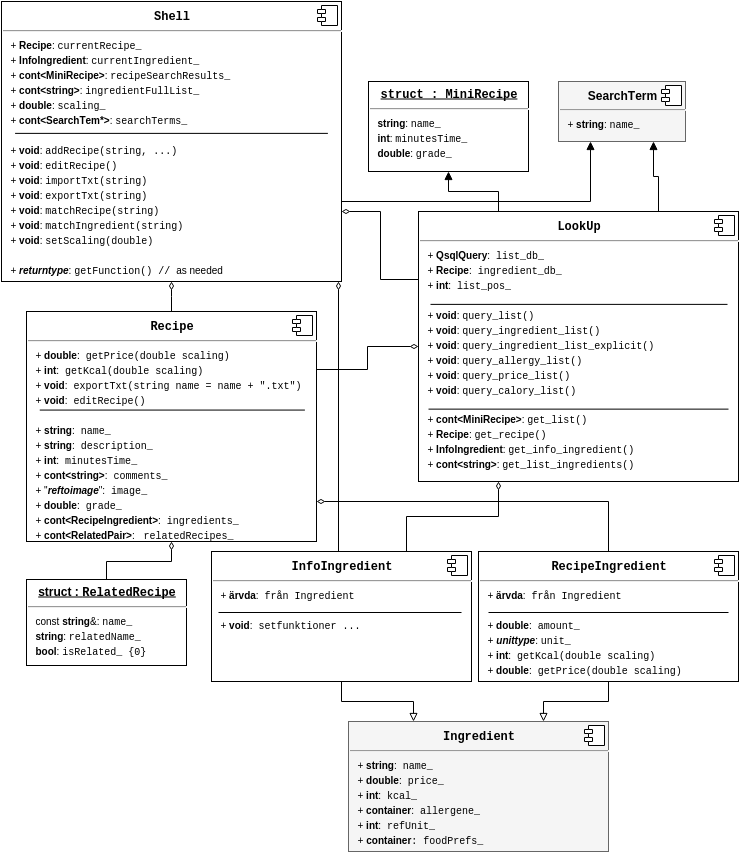
\includegraphics[width=16cm]{klass-schema.png}
\label{fig:classes}
\caption{Klass-schema}
\end{figure}

